\chapter{OpenShift私有容器云平台调度系统}
\label{cha:intro}
本章从Docker虚拟化技术出发,介绍在Docker基础上构建的三种典型集群管理系统: 一体式调度系统、两层调度系统和共享状态调度系统。分析了在Docker和容器编排管理器Kubernetes上构建的开源容器云平台OpenShift架构,其底层Kubernetes容器调度器的核心组件和调度原理。

\section{Docker虚拟化与OpenShift平台}
\label{sec:first}
\subsection{Docker虚拟化技术}
虚拟机是云计算的核心技术之一,以Docker为代表的容器虚拟化技术近几年大有取代虚拟机之势,逐步成为一种主流的技术。Docker是一种操作系统层面的虚拟化技术,其底层是LXC(Linux Container)作为支撑。和传统的虚拟技术面向操作系统或虚拟硬件不同,Docker是面向进程提供虚拟运行环境,其提供的虚拟环境就是容器。操作系统Linux可以为容器分配资源,如CPU时间、I/O时间、内存、外设访问控制等,并通过内核控制组(cgroups)子系统限定特定的进程使用资源的量,然后让Linux内核的namespace隔离容器间的进程。这样就可以实现一个高级的容器引擎,开发者可以快速构建、部署和发布应用,并且实现较好的跨平台。从资源管理角度而言,Docker依赖于LXC、LXC基于cgroups子系统,Docker主要是对容器进行封装,管理容器的生命周期、查询和控制相关信息、而所有与操作系统的交互都是通过libcontainer容器引擎完成。
\begin{figure}[H] % use float package if you want it here
	\centering
	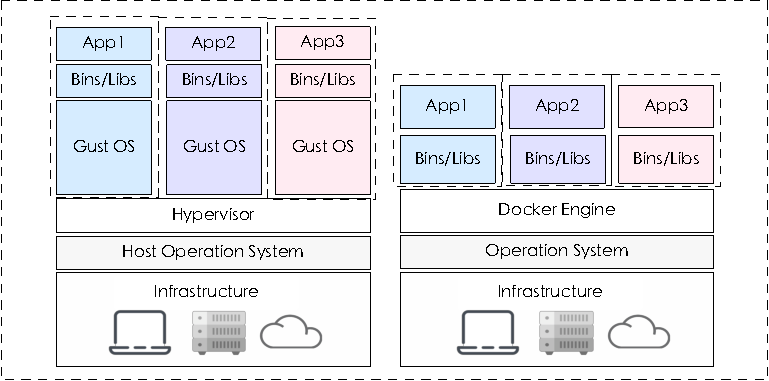
\includegraphics{docker-structure}
	\caption{容器与虚拟机对比}
	\label{fig:xfig1}
\end{figure}
图2-1中基础设施Infrastructure可以是个人电脑、服务器、云主机等,主机操作系统是运行在基础设施上的系统,最主要的是Linux各种版本,虚拟机管理系统(Hypervisor)可以实现在主机操作系统上独立运行多个子操作系统,在子操作系统上安装完应用所需的各种依赖后就可以实现资源应用的隔离。相对于虚拟机,Docker要简便很多,当前所有的Linux版本以及MacOS、Windows都能运行Docker,Docker Engine取代了Hypervisor,负载管理Docker容器并与操作系统通信,各种应用直接打包到镜像文件中,实现容器间的隔离。

对比Docker和虚拟机的架构发现,Docker直接通过守护进程与操作系统进行通信,管理容器并进行资源分配,实现容器与主操作系统的隔离。没有臃肿的子操作系统,各容器直接与主操作系统共享资源,节约了大量的磁盘空间,其虚拟化开销极大缩小,应用启动时间甚至达到毫秒级,用户可以快速构建、部署和交付应用,并且具有较强的跨平台性。
虽然Docker具有如此多的优势,但其隔离仅仅是在进程层面进行,并不能完全隔离整个运行环境。因此,用户需要根据自己的实际应用场景,需要彻底隔离用户的需求下选择虚拟机技术,如果仅是应用层面的隔离可以选择容器,如数据库、前端、后端等。
\subsection{OpenShift容器云平台}
\label{chap1:sample:table} 
Docker是当前主流的容器技术代表,Kubernetes作为现阶段应用最为广泛的容器编排引擎,OpenShift将这两种主流技术应用于企业,作为红帽公司提供的一款开源容器云平台。
该平台底层以Docker作为容器引擎驱动,Kubernetes作为容器编排组件,对外提供多种开发语言、中间件、数据库以及极易操作的用户界面、DevOps(Development and Operations)工具等。允许开发者和开发团队在该平台上进行应用的构建、测试、部署以及发布,是一套完整的容器应用云平台。在该平台上可以运行和支持有状态和无状态的应用;为容器应用提供较强的安全防护,包括基于用户的访问控制、检查机制以及强制隔离措施;实现多种综合云原生服务,便于快速智能、灵活开发应用、构建各种分布式系统;支持多种云环境包括Amazon Web Service、Azure、Google云平台以及VMware等;为开发运维团队提供一个通用的平台和工具,保持持续的开发和测试。OpenShift分为开源的社区版OpenShift Origin和收费的企业版OpenShift Enterprise,本文实验主要在开源的OpenShift Origin上进行分析和测试。
从技术堆栈的角度分析,OpenShift自下而上可以划分为基层架构层、容器引擎层、容器编排层、PaaS服务层、界面及工具层,如图2.2所示。下面分别对这几个层次进行介绍:
\begin{enumerate}[1.]
	\item 基础架构层。OpenShift运行所需的基础设施和环境,包括物理机、云主机、虚拟机、各种公有云、私有云以及混合云等。OpenShift支持多种操作系统,如CentOS7以上、Fedora21、Red Hat Enterprise Linux等,最后专门针对Atomic Host进行支持,是对企业版的Linux进行定制和优化的操作系统,可以为应用提供高度一致的运行环境,保证集群的稳定和安全。容器应用虽然具有较强的夸平台型,其前提是要求底层操作系统的内核和配置必须一致,因为其隔离依赖于Linux的内核。
	\item 容器引擎层。以当前主流的Docker作为OpenShift容器引擎,Docker已广泛应用于各种社区和环境中,经过了安全、稳定和高可用的检验。OpenShift并未修改任何原生的Docker代码,所有的应用最终到底层都生成一个Docker实例,只是将Docker的开放性和大量的镜像文件无缝衔接到平台上,对Docker的普通用户可以快速整合到平台中。
	\item 容器编排层。容器的编排对容器云的性能和资源利用效率具有决定性作用,OpenShift最终选择开源轻量的Kubernetes作为其容器编排引擎,Kubernetes已在Google内部使用多年,其诞生初衷就是为解决大规模集群中容器的调度和管理问题。OpenShift平台中很多基本的概念如Namespace、Pod、Replication Controller等都继承自Kubernetes,OpenShift同样只是将Kubernetes进行叠加使用,并未修改其原生代码和对象,用户依然可以通过原生的命令操作Kubernetes的对象。
	\item PaaS服务层。OpenShift在PaaS服务层提供了多种开发语言、框架、数据库以及中间件,极大提升了上层应用的开发、部署和交付速度。OpenShift有一个专门的社区以及Docker Hub提供各种应用的镜像,用户可以快速获取一个应用的基本镜像,构建自己所需的环,Red Hat的JBoss中间件几乎全部实现了容器化。
	\item 界面及工具层。OpenShift平台强大的界面及工具极大帮助普通用户高效完成相关应用业务,用户可以通过Web进行鼠标操作,平台将自动从Docker Hub中拉取所需的镜像进行应用构建,全自动化的服务极大降低了运维成本和提升服务效率。此外,OpenShift平台还提供S2I(Source to Image)服务,用户开发完成后可以自动整合到镜像中,快速实现交付,提升开发、测试、部署效率。针对用户端接入问题,平台提供Web控制台、IDE集成、命令行工具、以及RESTful API编程接口,用户可以最大限度的自由发挥。
\end{enumerate}
\begin{figure}[H] % use float package if you want it here
	\centering
	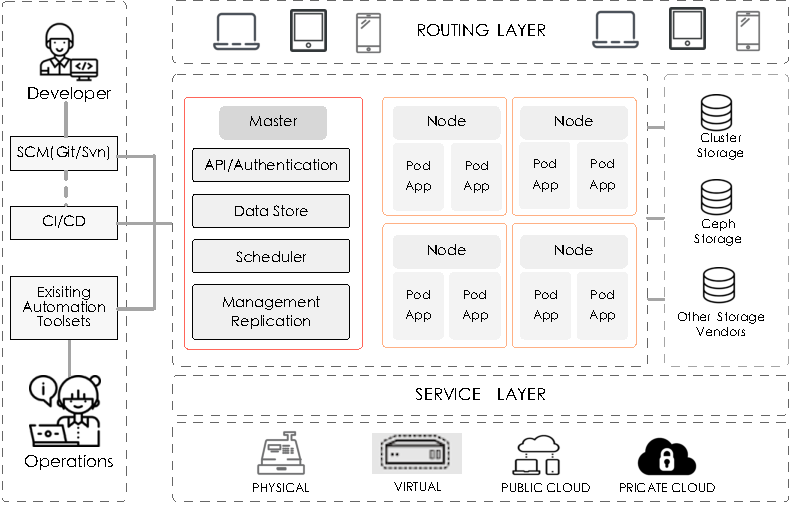
\includegraphics{openshift-structure}
	\caption{OpenShift Origin架构图}
	\label{fig:xfig1}
\end{figure}

如图2.2所示,OpenShift平台的核心组件包括Master、Node、Pod、Scheduler、Service、Storage等。Mater是主控节点,可以配置高可用的多个主控节点,负责管理和维护OpenShift集群的状态。Master上运行的API Server是其核心组件,所有用户的Web Console以及RESTful API服务都通过该组件进行访问认证控制,各Node节点也会定期轮询API Server更新其状态和容器的状态。Data Store将所有的状态信息存储在分布式的数据库Etcd中,并通过ceph一致性协议保证其数据的一致性,Etcd可以安装在主控节点,也可以单独安装到集群之外。Scheduler调度控制器进行Pod资源的分配和调度,收集过各节点资源情况,选择最优的节点作为容器应用的调度目标。Replication Controller异常自检测和恢复组件,负责监控集群中容器应用的状态和数量是否和用户要求一致,自启动和关闭容器应用满足用户的需求。Node节点通过接收Master节点指令维护容器应用。Pod是OpenShift平台调度器调度的最小单元,一些容器应用和应用之间往往存在较大的关联性,将几个联系紧密的容器部署在一个Pod中进行调度,提升应用的效率,如分布式数据库。容器是一个非持久化的对象,一旦容器重启或销毁,其状态信息将会随之销毁,集群每次给Pod分配的IP地址不同,要对外提供统一持久的服务,需要Service组件,该组件能将所有的信息转发到其对应的容器IP和端口上。此外,还有Router、Persistent Storage、Registry、Haproxy、Kubelet等都是集群的重要组成组件。数据的持久化存储可以是集群的数据库、分布式数据库或者其他的数据库中,当前支持的有NFS、Ceph RDB、GlusterFS等。

\section{容器集群资源调度系统}
\label{sec:scheduler}
Docker容器技术是容器集群的核心技术,但一个高效且强大的容器编排引擎也是集群的重要组成部分。一个好的调度器既要提现出作业调度的“公平”性,同时兼顾其性能和鲁棒性,要能应用的实际的生产环境中。在集群数据中心,可以通过应用对资源的需求感知用户部署的应用类型,通常可以划分为CPU密集、内存密集、I/O密集和网络带宽密集型应用。在集群上通常是多种密集型应用同时部署和运行,调度器如何进行资源分配至关重要,这就使得调度变得异常复杂和困难,往往不存在最优解决方案。传统虚拟机的云计算中心资源调度已有相当多的研究,针对容器集群,各大容器产生也相继推出了几款优秀的容器编排引擎,根据其调度架构的不同可以划分为一体式调度系统、两层调度系统、共享状态调度系统。其代表分别是Docker公司的Swarm、Apache的Mesos、Google的Kubernetes。

\subsection{一体式调度系统}
一体式的调度使用单一的调度代理处理所有的请求,通过固定的调度算法调度所有的作业,这种调度方式导致调度扩展性很差,用户很难灵活定制自己的调度策略,而且所有的调度信息在单节点上进行运算,不能并行执行,单节点也会成为其瓶颈。Docker公司2014年发布的容器编排管理工具Swarm是典型的一体式调度系统,同期发布的还有Docker管理工具Machine以及Compose,合称为Docker三剑客。Swarm支持Docker标准的API,内置于Docker CLI中,无需进行安装,拥有活跃的社区,易于搭建并且已应用于实际的生产环境中。
\begin{figure}[H] % use float package if you want it here
	\centering
	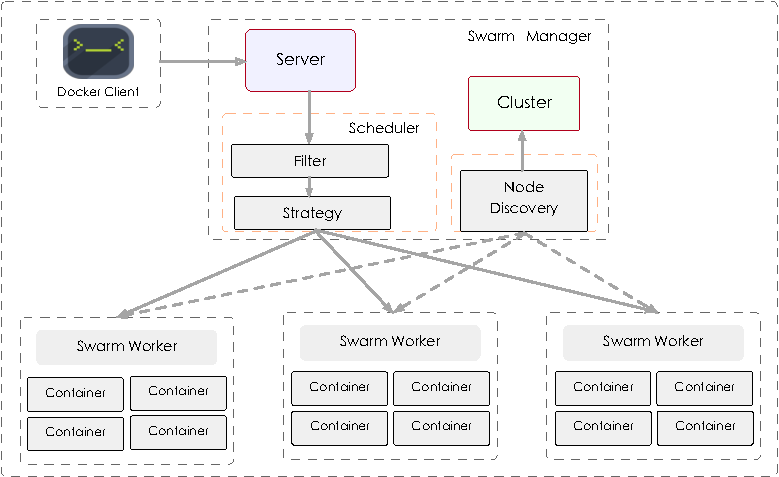
\includegraphics{swarm-structure}
	\caption{Swarm架构图}
	\label{fig:xfig1}
\end{figure}

Swarm集群由管理节点和工作节点构成,其中管理节点可以配置多个,实现高可用的多管理模式,内部通过RAFT算法实现主从的一致性。管理节点上除Docker Daemon守护进程、Load Balancing、Scaling组件外,最为重要的是Scheduler和Discovery组件,其中Discovery负责集群中节点的发现和状态更新,Scheduler首先根据用户的限制对节点进行筛选,然后使用内置的调度策略进行应用调度。工作节点主要运行Docker Daemon和Load Balancing,根据控制节点的指令运行调度过来的容器应用。在调度器的过滤模块主要提供了约束过滤器和健康过滤器,此外还可以配置吸引力过滤器、依赖过滤器和端口过滤器。

约束过滤器是通过有用的约束条件筛选节点,集群中每个节点都带有一个key-value标签,对于一些特殊的应用可以指定其label进行调度到指定的节点上运行;健康过滤器过滤掉不健康的节点,避免容器调度后运行失败;吸引力过滤器是将新的容器链接到已经创建的容器上,实现共同运行和销毁,此外还可以通过镜像和标签吸引,镜像吸引是将容器直接调度到拥有该镜像的节点上,避免重复开销镜像下载时间,节约网络资源,标签吸引是通过标签指定链接到已创建的旧容器实现共同工作;依赖过滤器是新容器依赖于其他的容器,可能会共享磁盘卷、或在同一个网络栈上等;端口过滤器将需要特定开发端口的容器运行到开放该端口的节点上,避免容器不可用的情况发生。

Swarm的调度策略主要包括Random、Spread和Binpack算法,下面分别对其算法进行简单的介绍:
\begin{enumerate}[1.]
	\item Random算法。该算法随机从过滤完的节点中选取一个节点进行调度判断,如果该节点满足条件则将容器调度到该节点上,否则随机选取下一个节点直至找到合适的节点调度,直至找到合适的节点或返回调度错误信息。
	\item Spread算法也就是最少容器算法,该算法的初衷是保证容器进群的负载均衡。每次遍历一遍集群中每个节点上运行的容器数量,选择容器数量最少的节点进行容器调度,若该节点不满足条件,则依次从后往前进行调度尝试,直至找到满足条件的节点或返回调度错误。
	\item Binpack算法就是最多容器算法,该算法的目的在于最大化利用集群中节点资源,和Spread算法相反,每次从集群中选择运行容器数量最多的节点进行容器调度,若满足条件则将容器调度至该节点,否则依次从多到少尝试运行容器节点,直至找到合适节点或返回错误。
\end{enumerate}

\subsection{两层调度系统}
两层调度系统是将资源调度和作业调度分开,资源调度层只负责给计算框架分配所需的资源,具体的作业调度由每个计算框架的调度算法完成。在一些成熟的计算处理框架中如Hadoop、Spark、MPI等有相对成熟和高效的调度算法,两层调度将这些调度算法集成进来,通过一个轻量的资源共方式来控制资源的分配和访问,一旦资源分配给某个计算框架,其他计算框架不能使用该资源,因此也会造成资源利用效率不高。Apache Mesos是最为典型的两层调度系统,Mesos最初由加州伯克利分校的AMPLab开发,后在Twitter得到广泛使用和检验。

\begin{figure}[H] % use float package if you want it here
	\centering
	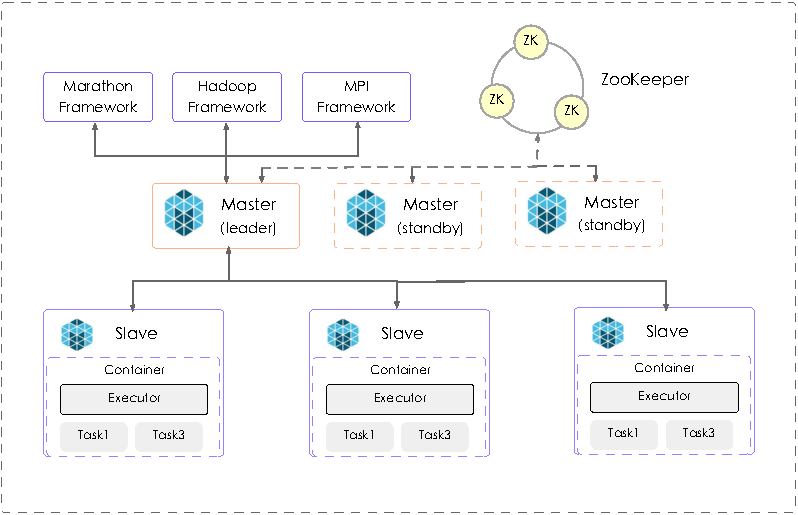
\includegraphics{mesos-structure}
	\caption{Apache Mesos架构图}
	\label{fig:xfig1}
\end{figure}

如图2.4所示,Mesos的总体架构也采用主从设计,Master节点运行作为集群的管理控制节点,可以有一个或者多个(最好为单数),为了防止单节点故障,通过ZooKeeper提供一致性服务。每次在多个Master中选举一个作为leader对外提供服务,其他的Master副本随时保证和Master的状态一直,一旦服务出现故障,立马进行新的备份选举,从而实现集群的高可用性。集群的架构可以分为两层: 计算框架层和Master调度层。下层的Master管理众多的计算节点,负责收集各节点的资源情况并作出分配决定,上层的计算框架层负责实际任务的调度,从而将整个调度分为了任务调度层和资源调度层,两个层级互不干扰,可以分别使用调度算法,提升了集群调度策略的扩展性。从架构的组成部分来看,主要有五大组成部分,下面分别对组成部分的功能进行介绍:
\begin{enumerate}[1.]
	\item ZooKeeper组件。ZooKeeper作为一款Hadoop项目中分布式系统的协调系统,主要用于解决分布式应用中数据管理问题,如应用配置管理、统一命名服务、状态同步服务以及其他的组服务、集群管理等。ZooKeeper操作非常简单易用、功能丰富可靠、并且提供了通用协议下的开源共享的存储库,其核心就是一个精简的文件系统,可以提供一些简单和抽象的操作。在Mesos中、ZooKeeper主要解决Master节点的状态一致性和高可用问题,实现集群的持续稳定的对外服务。
	\item Mesos Master组件。Master是整个集群的控制器,是整个集群调度的核心组件,既需要对底层的各Slave节点的资源进行管理和收集,同时通过一定的资源分配策略提供资源个体上层的各处理框架Framework。当前对各Framework的资源分配策略为DRF(Dominant Resource Fairness)算法,这是一种针对多维资源(CPU、内存、I/O、网络带宽等)不同需求设计的公平调度算法
	。Master还负责资源的访问控制,一旦某个资源分配给了特定的Framework,必须等该框架释放该资源才能再次进行分配。
	\item Mesos Slave组件。该组件作为调度底层具体的执行者,接收来自Master的指令,将自身的资源分配给每个执行器,执行器上运行一个或多个任务,并将各任务作为容器运行起来。
	此外,Slave节点还定期向Master节点汇报资源使用情况作为Master调度器的调度依据。Slave上还运行一个containerizer用来管理容器的生命周期的包括容器的创建、更新、监控和销毁。
	\item Framework组件。Framework负责将各计算框架如Hadoop、Spark、MPI等注册接入到集群中,Master的调度器负责对其需要的资源进行分配,具体的任务调度则由各计算框架完成。
	各计算框架通过调用Master的API进行任务的创建和调度请求,Master再将任务下发到Slave上具体执行。
	\item Executor组件。Executor负责启动框架内部的Task任务,各种计算框架接入Mesos的方式,接口不同,因此要接入一个新的计算框架就需要编写一个新的Executor,用来通知Mesos如何启动框架中的Task任务。
\end{enumerate}

Mesos作为一款优秀的分布式资源管理框架,采用双层调度机制,资源分配层负责将资源分配给计算框架,计算框架使用自身的任务调度器执行任务的调度。通过对其整体建构和核心组件的分析,Mesos可以对分布式集群的资源进行细粒度的划分,按照计算框架实际任务的需求进行资源分配,极大提升了资源的利用效率。Mesos不需要清楚各Framework的具体调度逻辑,只需要通过API向上提供资源分配即可,具有较强的扩展性,容量不会成为制约其性能的因素。Meso是模块化的实现,新增一个Framework不需要对Mesos进行重新编码,可以快速接入和扩展新的应用,Master节点使用ZooKeeper保证其状态一致性,容错性很好。但是,Mesos对底层的资源采用“悲观锁”的方式进行控制,一旦被某个Framework占用,必须等到其释放才能进行新的资源分配,其并发性受到极大的限制,独立的调度框架只能访问集群部分状态信息,往往不能实现优化调度。
\subsection{共享状态调度系统}
在一体式调度系统中,资源分配和任务调度都由中心调度器进行管理,并且集成了具体的调度算法;在两层调度系统中,资源分配由资源调度层完成,任务调度由具体的计算框架自己完成。一体式的调度很好的保证了全局状态的一致性,但是扩展性较差,两层调度系统虽然扩展性姮好,但是集群状态的一致性较难保证,并且容易造成资源的竞争和死锁。为了解决这些不足,共享状态调度系统被提了出来,其核心在于所有的调度逻辑共享集群状态,选择最优的节点进行资源分配和任务调度。其中最为典型就是Google推出的Borg、Kubernetes以及使用事务方式解决一致性管理问题的Omega,其中Kubernetes以其开源性深受大众好评,各大主流的互联公司都加大对其支持力度。

\begin{figure}[H] % use float package if you want it here
	\centering
	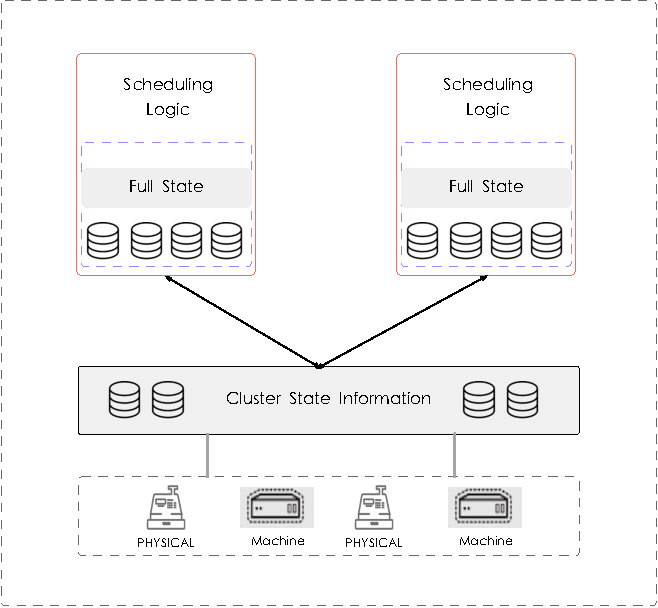
\includegraphics{full-state-structure}
	\caption{共享状态资源调度系统}
	\label{fig:xfig1}
\end{figure}
在共享状态调度系统中,每一个上层的调度器都可以对整个集群的状态进行访问,资源对所有的调度器都是透明的,可以实现自由竞争,不存在单一的资源分配器,因此也不存在单一节点访问瓶颈。集群不仅支持节点资源的快速增加,也支持调度器的扩展,用户根据自己的实际应用场景开发特殊的调度器,可以很轻易的集成到集群中。为了保证集群的高并发性和可扩展性,共享状态调度系统采用“乐观锁”对底层资源进行并发控制。具体的实现是通过对集群的所有状态都增加一个版本属性,每次提交时比较提交的版本和当前版本号大小,若版本号小于当前的版本号,则不进行任何处理,只有提交版本号大于当前数据版本号的操作才被接受,更新完状态后版本号递增。“乐观锁”并发控制虽然会增加资源访问的冲突数,影响系统的吞吐率,但在实际的系统中依然在一个可以接受范围,下一个小节将对Kubernetes调度系统架构和流程做详细的分析。

\section{Kubernetes资源调度系统}
\label{sec:bib}
Kubernetes是典型的基于共享状态的调度系统,是一个轻量的开源平台,用于容器化应用管理和服务,使用Label和Pod的概念将容器划分为逻辑单元,将相关容器进行共同调度和部署。针对其核心组件和整体架构进行深入的分析,尤其是对其调度算法和不足进行研究,为下一步提出新的调度方案提供依据。
\subsection{Kubernetes简介}
Kubernetes源自Google的Borg项目,Borg是Google集群管理工具,稳定地管理全球上百万台服务器多年。为了在容器云竞争中占据领导地位,Google基于Borg的管理经验,研发了基于Docker的容器编排工具Kubernetes,并在2014年将其开源,逐步形成一个大的生态。作为一个跨主机的应用容器编排引擎,Kubernetes提供了一系列完整的功能,包括应用部署运行、资源调度、服务发现、动态扩容以及错误恢复等。Kubernetes同时具备强大的集群管理能支撑分布式系统,实现了多租户应用、服务发现和服务注册、负载均衡、故障自处理和恢复、在线扩容、细粒度调度、资源配额管理等功能,完整定义了构建业务系统的标准化架构层。除集群管理方面的强大功能外,Kubernetes还提供完整的开发、测试、部署、运维监控在内各个环节的工具。

Kubernetes逐步发展成一个巨大生态圈,为容器的编排提供一个简单、轻量的方式,最重要的是用户可以开源定制。当前支持采用Kubernetes的云计算服务商和用户越来越多,如微软、Yahoo、IBM、华为、VMware、网易、阿里、华为、亚新等,甚至一些初创公司灵雀云、青云等都采用Kubernetes作为容器云的管理系统。

Kubernetes拥有强大而活跃的社区,众多开发者不断对其进行迭代更新,其代码更加完善。当前支持Kubernetes社区的支持者有Google、CoreOS、RedHat、华为、网易、阿里云、浙大SEL实验等。Google在2015年联合其他20多家公司成立了开源组织CNCF(Cloud Native Computing Foundation),加入OpenStack社区,力推Kubernetes的广泛应用,支持其在当前公有云、私有云等各种基础设施平台上运行,提供更加简便丰富的工具集,更好的服务用户。

\subsection{Kubernetes架构和组件}


\section{公式}
\label{sec:equation}
贝叶斯公式如式~(\ref{equ:chap1:bayes}),其中 $p(y|\mathbf{x})$ 为后验;
$p(\mathbf{x})$ 为先验;分母 $p(\mathbf{x})$ 为归一化因子。
\begin{equation}
\label{equ:chap1:bayes}
p(y|\mathbf{x}) = \frac{p(\mathbf{x},y)}{p(\mathbf{x})}=
\frac{p(\mathbf{x}|y)p(y)}{p(\mathbf{x})} 
\end{equation}

论文里面公式越多,\TeX{} 就越 happy。再看一个 \pkg{amsmath} 的例子:
\newcommand{\envert}[1]{\left\lvert#1\right\rvert} 
\begin{equation}\label{detK2}
\det\mathbf{K}(t=1,t_1,\dots,t_n)=\sum_{I\in\mathbf{n}}(-1)^{\envert{I}}
\prod_{i\in I}t_i\prod_{j\in I}(D_j+\lambda_jt_j)\det\mathbf{A}
^{(\lambda)}(\overline{I}|\overline{I})=0.
\end{equation} 

前面定理示例部分列举了很多公式环境,可以说把常见的情况都覆盖了,大家在写公式的时
候一定要好好看 \pkg{amsmath} 的文档,并参考模板中的用法:
\begin{multline*}%\tag{[b]} % 这个出现在索引中的
\int_a^b\biggl\{\int_a^b[f(x)^2g(y)^2+f(y)^2g(x)^2]
 -2f(x)g(x)f(y)g(y)\,dx\biggr\}\,dy \\
 =\int_a^b\biggl\{g(y)^2\int_a^bf^2+f(y)^2
  \int_a^b g^2-2f(y)g(y)\int_a^b fg\biggr\}\,dy
\end{multline*}

其实还可以看看这个多级规划:
\begin{equation}\label{bilevel}
\left\{\begin{array}{l}
\max\limits_{{\mbox{\footnotesize\boldmath $x$}}} F(x,y_1^*,y_2^*,\cdots,y_m^*)\\[0.2cm]
\mbox{subject to:}\\[0.1cm]
\qquad G(x)\le 0\\[0.1cm]
\qquad(y_1^*,y_2^*,\cdots,y_m^*)\mbox{ solves problems }(i=1,2,\cdots,m)\\[0.1cm]
\qquad\left\{\begin{array}{l}
    \max\limits_{{\mbox{\footnotesize\boldmath $y_i$}}}f_i(x,y_1,y_2,\cdots,y_m)\\[0.2cm]
    \mbox{subject to:}\\[0.1cm]
    \qquad g_i(x,y_1,y_2,\cdots,y_m)\le 0.
    \end{array}\right.
\end{array}\right.
\end{equation}
这些跟规划相关的公式都来自于刘宝碇老师《不确定规划》的课件。
